% ----------------------------------------------------------
% Introdução
% ----------------------------------------------------------
\chapter[Introdução]{Introdução}
No Brasil temos muitos casos de abandonos de animais. Em 2019 o Instituto Pet Brasil realizou um levantamento a respeito de animais sob tutela de \ac{ONGs}, e chegaram ao resultado de mais de 170 mil animais. Desses, 96\% são cachorros e apenas 4\% são gatos. Além das \ac{ONGs} muitas pessoas resgatam animais que encontram na rua em situações de vulnerabilidade, levam para suas casas e fornecem lares temporários até encontrarem, então, uma família que possa oferecer todo cuidado que o animal necessita \cite{tutelaONG}.

O ano de 2020 foi marcado pela pandemia da \gls{COVID-19}, devido a isso, a população foi submetida a um período de quarentena obrigatória. Nos primeiros meses, com mais tempo em casa, os brasileiros recorreram a \ac{ONGs} em busca de companhia animal, aumentando os números de adoções \cite{adocao}.

O país foi afetado em diversas questões: econômica, social, política e culturalmente, causando, assim, uma reviravolta na vida de todos, inclusive dos animais. Novamente o índice de abandono cresce, e com alguns fatores como desemprego em grandes níveis, retorno de atividades presenciais, fim do auxílio emergencial, o cuidado dos amimais ficou inviável para alguns tutores \cite{abandono_pandemia}. 

Visando facilitar o processo de adoção, tanto para o adotante, como para o doador, a equipe TI TI TI decidiu por desenvolver um \textit{website} que atendesse às necessidades dos usuários, possibilitando a busca por um animal que combine com as premissas do adotante.

\section{Problema a ser solucionado}
Em 2013 a \ac{OMS} lançou uma nota que continha estimativas do número de animas vivendo nas ruas do Brasil, eram cerca de 20 milhões de cães e 10 milhões de gatos. Em cidades grandes como São Paulo e Rio de Janeiro há um cachorro a cada 5 habitantes, e 10\% destes não tem um lar.

Com o início da pandemia e confinamento brasileiro, as \ac{ONGs} passaram a reportar um aumento na procura de adoção de cães e gatos. Segundo o médico veterinário que é gerente de vigilância do \ac{CCZ} do Distrito Federal, Rodrigo Menna Barreto, o número de adoções de animais registrados pelo órgão entre janeiro e setembro de 2020 foi maior que o dobro registrado em todo o ano anterior.

Infelizmente essa rara notícia boa não durou, quando a pandemia passou a viver seu pior momento no Brasil com crise social e econômica, muitos dos animais voltaram ao seu destino anterior sendo abandonados ou devolvidos por famílias que alegaram falta de condições financeiras ou psicológicas para cria-los, além daqueles que os abandonavam por medo de ter \gls{COVID-19} por transmissão de cães e/ou gatos (uma informação comprovada falsa). Isso levou a \ac{ONGs} superlotadas e recordes de abandono.

\section{Justificativa}
Diariamente ao sairmos de nossas casas, cenas de cães e gatos abandonados são muito comuns, principalmente em centros urbanos, onde reside a maior parte da população. Na pandemia é notável que essas cenas acabaram ficando cada vez mais frequente, tornando a reflexão acerca do tema um tanto relevante.

De acordo com dados da \gls{AMPARA}, cerca de 60\% a 70\% de animais foram abandonados, entre julho de 2020 e fevereiro de 2021 (em comparação com 2019). Um dos muitos motivos para tal estimativa é a dificuldade financeira, e adoção por impulso durante o período de quarentena \cite{abandono}.

Em vista de tais dados, nossa equipe se sensibilizou com a causa e decidiu criar um projeto que realize a adoção de cães e gatos de forma prática e efetiva, contribuindo, dessa forma, com a diminuição dos números de abandonos, de maneira consciente e solidária.

\section{Objetivos}

A equipe TI TI TI desenvolveu o \textit{website} PETINDER visando prover para os usuários da plataforma um local seguro onde possa acontecer a conexão entre animal e adotante. Temos como objetivo também auxiliar na queda dos números de animais em situação de rua e ajudar cães e gatos a encontrarem novos lares onde possam receber proteção e afeto.

O projeto tem como objetivos específicos:

\begin{itemize}
\item Facilitar o processo de adoção de cães e gatos;
\item Oferecer uma plataforma segura e intuitiva para o usuário;
\item Colaborar com a diminuição do número de animais abandonados do país.
\end{itemize}

% ---
% Capitulo de revisão de literatura
% ---
\chapter{Revisão da Literatura}
A revisão da literatura é a etapa do trabalho em que se reúne as fontes de pesquisa que vão fornecer embasamento teórico para o trabalho.

Além disso, serve para dialogar com essas referências e aplicar seus conceitos no tema da monografia.

Portanto, é na revisão da literatura onde deve-se apresentar um levantamento bibliográfico acerca do assunto que será tratado na monografia, com escopo definido e uma análise crítica sobre os autores selecionados. 

%Todos trabalhos devem possuir a revisão de literatura onde são abordados os estudos feitos com base da literatura (livros, artigos acadêmicos, publicações em periódicos), todos elementos devem ser referenciados por citações.

%Não são abordados aqui itens técnicos que normalmente são vistos em disciplinas anteriores do curso (UML, banco de dados, metodologias de gerenciamento de projeto etc...)

\section{Assunto X}

\chapter{Descrição funcional da aplicação}
% Falar das funcionalidades da aplicacao, das partes interessadas, e dos concorrentes (incluir tabela de comparacao)

\section{Casos de uso}
% Descricao e diagrama

\chapter{Modelagem e levantamento de dados}
O presente capítulo dispõe-se de especificar os dados e revelar as modelagens e os diagramas construídos para fins de instrução de quem o usufruir como é mostrado nos \autoref{quadro-rf} e \autoref{quadro-rnf} onde estão localizados os requisitos para uso do PETINDER de forma adequada , e também no desenvolvimento da arquitetura do \textit{website}, que é apresentado nas \autoref{mer} e \autoref{der} respectivamente. Sendo assim, foi detalhado nos subcapítulos todos os modelos e diagramas que criamos, e a descrição dos mesmos.
% Falar do uso do modelo MVC e aplicacao no projeto (incluir modelo de classes, modelo do banco


\section{Análise de Requisitos}
Na engenharia de \textit{software}, mais precisamente na engenharia de requisitos (comumente chamada apenas de Análise ou Levantamento de Requisitos) é a disciplina que identifica a “dor” do cliente, faz um “diagnóstico” sobre sua origem e propõem um “tratamento terapêutico” para curá-lo \cite{analise}.

\subsection{Requisitos funcionais}
Requisitos funcionais são todas as necessidades, características ou funcionalidades esperadas em um processo que podem ser atendidos pelo \textit{software} \cite{analise}.

De forma geral, um requisito funcional expressa uma ação que deve ser realizada através do sistema, ou seja, um requisito funcional é “o que sistema DEVE fazer”.  No \autoref{quadro-rf} estão os requisitos funcionais da aplicação PETINDER.

\begin{quadro}[htb]
\centering
\caption[Requisitos funcionais]{Requisitos funcionais}
\label{quadro-rf}
\begin{tabular}{|p{1.6cm}|p{10.2cm}|p{2.2cm}|}

\hline     
\thead{Código} & \thead{Descrição} & Requisito Relacionado\\ 
\hline                               
RF01 & O sistema deve permitir o cadastro de usuários que pretendem adotar e/ou doar cães e gatos. & \\
\hline     
RF02 & O sistema deve permitir o cadastro de animais.& \\
\hline     
RF03 & O sistema deve permitir um controle de informações dos animais cadastrados para um tutor. & RF02\\
\hline     
RF04 & O sistema deve apresentar a quantidade de animais cadastrados pelo tutor em sua conta. & RF02\\
\hline 
RF05 & O sistema deve permitir que um adotante demonstre interesse em um animal por meio do \gls{Miau-dorei}. & \\
\hline 
RF06 & O sistema deve apresentar as informações dos adotantes interessados pelos animais aos seus doadores. & \\
\hline 
RF07 & O sistema deve permitir que doador demonstre interesse no adotante por meio do \gls{Miau-dorei}. & \\
\hline 
RF08 & Quando o \gls{Miau-dorei} é mútuo entre doador e adotante o sistema deve notificar o \gls{Match}. & RF05\\
\hline 
RF09 & O sistema deve permitir a interação entre doador e adotante através do \textit{chat} após o \gls{Match}. & \\
\hline 
RF10 & O \textit{chat} do sistema deve mostrar hora e data das mensagens trocadas entre usuários. & RF09\\
\hline 
RF11 & Os adotantes que demonstrarem interesse em um animal com \textit{status} “em processo de adoção” serão direcionados a uma fila de espera para caso a adoção anterior não seja concluída. & RF08\\
\hline     
\end{tabular}
\fonte{Elaborada pelos autores}
\end{quadro}


\subsection{Requisitos não funcionais}
Um requisito não funcional, pode ser definido como “de qual maneira” o sistema deve fazer algo. Por outro lado, pode parecer muito vago e com pouco sentido, mas é muito simples assimilar o conceito.

Uma forma simples de entender o que é um requisito funcional é ter por base que todo requisito não funcional deve expressar uma premissa ou restrição do sistema \cite{analise}. No \autoref{quadro-rnf} estão os requisitos não funcionais da aplicação PETINDER.

\begin{quadro}[htb]
\centering
\ABNTEXfontereduzida
\caption[Requisitos não funcionais]{Requisitos não funcionais}
\label{quadro-rnf}
\begin{tabular}{|p{1.6cm}|p{12.4cm}|}

\hline     
\thead{Código} & \thead{Descrição}  \\ 
\hline                               
RNF01 & Para utilizar o sistema o usuário precisa estar conectado a uma rede Wi-Fi ou dados móveis.\\
\hline     
RNF02 & Bcrypt será utilizado para segurança de senhas inseridas no sistema.\\
\hline     
RNF03 & O sistema deverá ter interligação com o banco de dados PostgreSQL. \\
\hline     
RNF04 & O sistema deverá ser desenvolvido para \textit{website}.\\
\hline     
\end{tabular}
\fonte{Elaborada pelos autores}
\end{quadro}

\subsection{Regras de negócio}
Regras de negócio servem para definir ou restringir alguma ação nos processos de sua empresa.

São declarações que irão descrever como determinadas operações devem ser realizadas e se há algum limite que precisa ser aplicado. São elas que guiarão comportamentos e definirão o que, onde, quando, porque e como algo deve ser feito em uma empresa. No \autoref{quadro-rn} estão as regras de negócio da aplicação PETINDER \cite{regras}.

\begin{quadro}[!htbp]
\centering
\ABNTEXfontereduzida
\caption[Regras de negócio]{Regras de negócio}
\label{quadro-rn}
\begin{tabular}{|p{1.6cm}|p{12.4cm}|}

\hline     
\thead{Código} & \thead{Descrição} \\ 
\hline                               
RN01 & Os animais cadastrados no sistema devem ser exclusivamente para adoção.\\
\hline     
RN02 & Os animais cadastrados deverão ser apenas gatos e cachorros.\\
\hline     
RN03 & Os usuários podem atuar como adotantes e/ou doadores de animais no  sistema. \\
\hline     
RN04 & O \textit{chat} do sistema deve ser usado para seus devidos fins de adoção de animais. O PETINDER contará com um sistema de denúncias para os usuários.\\
\hline     
RN05 & Denúncias avaliadas pelos administradores do sistema como verdadeiras geram uma infração para o perfil denunciado.\\
\hline     
RN06 & Caso um mesmo usuário cometa três infrações ele será banido temporariamente do sistema, se uma mesma conta for banida três vezes, ela será excluída permanentemente.\\
\hline     
RN07 & Os administradores do sistema não se responsabilizam por problemas relacionados à utilização de nossas ferramentas.\\
\hline     
RN08 & Os administradores do sistema não se responsabilizam pela saúde e/ou cuidados com os animais cadastrados.\\
\hline     
RN09 & Qualquer usuário pode ver a listagem de animais cadastrados no sistema.\\
\hline     
RN10 & Quando um usuário adota um animal ele adquire tutoria dos dados de cadastro do animal.\\
\hline     
RN11 & O usuário tem a opção de desfazer um \gls{Des-au-gostei}.\\
\hline     
RN12 & Caso um usuário não-logado tente interagir com as funções de adoção e/ou doação ele será redirecionado a tela de \textit{login}.\\
\hline     
\end{tabular}
\fonte{Elaborada pelos autores}
\end{quadro}

\clearpage
%---------------------------------------------
\section{Casos de uso}
% Descricao e diagrama
O diagrama de casos de uso documenta o que o sistema faz a partir do ponto de vista do usuário, ou seja, ele descreve as principais funcionalidades do sistema e a interação dessas funcionalidades com os usuários do mesmo sistema. Nesse diagrama não nos aprofundamos em detalhes técnicos que dizem como o sistema realiza essas funções \cite{caso}.

\begin{figure}[!htbp]
    \centering
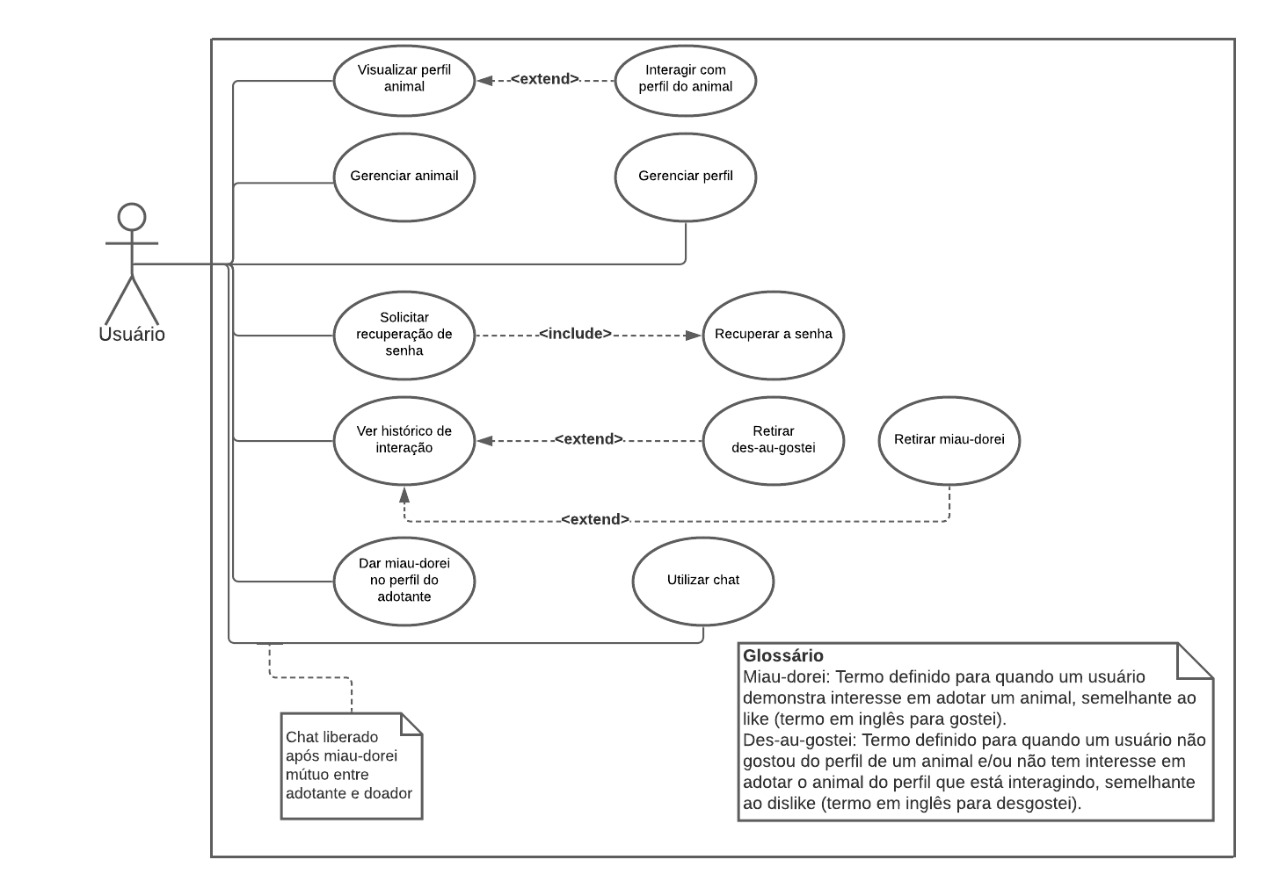
\includegraphics[scale=0.4,angle=90]{imagens/CasosDeUsoPETINDER.jpeg}
	\caption{\label{diagama-casos}Diagrama de Casos de Uso do Sistema}
	\fonte{Elaborada pelos autores}
\end{figure}

\section{Tecnologias utilizadas}
As tecnologias definitivas utilizadas pela equipe no projeto foram determinadas  na \ac{POC}, assim como mostra o \autoref{provaconceitual-pdfpages}.  
\subsection{Para a aplicação}
\ac{HTML}: é uma linguagem de marcação de hipertexto para apresentar e estruturar o conteúdo na \textit{web} \cite{html}.

\ac{CSS}: é uma "folha de estilo" composta por “camadas” e utilizada para definir a apresentação (aparência) em páginas da \textit{internet} que adotam para o seu desenvolvimento linguagens de marcação \cite{css}.

JavaScript: é uma linguagem de programação criada em 1995 por Brendan Eich enquanto trabalhava na Netscape Communications Corporation \cite{jsum}. É uma linguagem de programação de alta complexidade, mas de fácil uso, voltada para criar elementos em aplicações \textit{web}, como sites, aplicativos e sistemas \textit{online} \cite{jsdois}. 
Durante o desenvolvimento foi utilizada uma \ac{API} da tecnologia, denominada "GeoLocation", a qual possibilita acessar a localização do usuário em tempo real.

Bootstrap 5: foi inicialmente criado por Mark Otto e Jacob Thornton para o desenvolvimento web mais rápido e prático. Ele contém todos os tipos de templates baseados em HTML e CSS para várias funções e componentes. Por exemplo: navegação, sistema de grades, carrosséis de imagens e botões. A lista não é exaustiva.  \cite{bootstrap}.

\ac{PHP} é uma linguagem de programação utilizada por programadores e desenvolvedores para construir sites dinâmicos, extensões de integração de aplicações e agilizar no desenvolvimento de um sistema \cite{php}.

CodeIgniter: esse \textit{framework} de desenvolvimento de aplicações, se compararmos com outros, disponibiliza um conjunto de classes que podem ser combinados e estendidos para que aplicações sejam construídas, nos poupando um considerável tempo de codificação \cite{codeigniter}.
Durante o desenvolvimento foram utilizadas bibliotecas do \textit{framework}, como a de envio de e-mail através do protocolo \ac{SMTP}, a de validação de formulários e a de \textit{upload} de imagens. Além disso, também foi utilizada a biblioteca de testes unitários disponível no \gls{CodeIgniter} para realizar os testes automatizados da aplicação, assim como consta no \autoref{testes}.

Visual Studio Code: é um editor de código-fonte leve desenvolvido pela Microsoft. Possui as funcionalidades mais simples como: edição de código com suporte a várias linguagens de programação, terminal de comandos integrado e controle de versão \cite{vscode}.

PostgreSQL: é um \ac{SGBDOR}, desenvolvido como projeto \textit{software} livre, é de código e conta com recursos como: consultas complexas, chaves estrangeiras, integridade transacional, controle de concorrência multi-versão, suporte ao modelo híbrido objeto-relacional, \textit{trigger}, \textit{views} e \textit{stored procedures} em várias linguagens \cite{postgresql}.

PostGIS: é uma extensão geoespacial para o \ac{SGBDOR} \gls{PostgreSQL}. Este módulo é uma robusta solução para o suporte ao armazenamento, gerenciamento, tratamento e análise de dados espaciais \cite{postgis}.

Leaflet: É uma biblioteca JavaScript de código aberto para mapas interativos compatíveis com dispositivos móveis. Pesando apenas cerca de 39 KB de JS, ela tem todos os recursos de mapeamento que a maioria dos desenvolvedores precisa \cite{mapa}.

Azure: É uma plataforma da Microsoft formada por uma série de ferramentas diferentes que libera o acesso a empresas e desenvolvedores, a capacidades de processamento e armazenamento dos \textit{datacenters} da Microsoft. O projeto PETINDER foi hospedado na plataforma Azure. O \ac{IFSP} disponibiliza aos alunos um convênio para assinatura estudantil que fornece créditos que podem ser utilizados na plataforma. A equipe optou por esse serviço de hospedagem pelos seguintes fatores: certificado \ac{SSL} com nota A (\autoref{teste-ssl} e o acesso ao bando de dados \gls{PostgreSQL} e sua extensão geoespacial \gls{PostGIS} \cite{azure}.

\subsection{Requisitadas pela disciplina}
Subversion: é uma ferramenta de controle e versionamento. A equipe utilizou para compartilhar as versões mais recentes da aplicação e da documentação.

\LaTeX:  é um sistema ou programa de marcação para a editoração de documentos de alta qualidade tipográfica, específico para a elaboração de textos científicos. Trata-se de um conjunto de macros ou marcações para o processador de textos TeX \cite{latex}.

YouTube: o site surgiu em virtude do inconveniente que era compartilhar arquivos de vídeo, já que estes eram muito grandes, o que dificultava seu envio por e-mail. O site permite que os usuários coloquem seus próprios vídeos na rede, sendo visualizados por qualquer pessoa no mundo inteiro \cite{youtube}. A equipe utilizou desta tecnologia para postar os vídeos solicitados pela disciplina.

Blogger: é a plataforma gratuita de \textit{blogs} do Google. Além de ser fácil de navegar e administrar, oferece a hospedagem e diversos recursos que permitem ao usuário criar seu \textit{blogs} e personalizá-lo, de acordo com suas necessidades \cite{blogger}. A equipe utilizou desta tecnologia para postar relatórios semanais  solicitados pela disciplina.

%---------------------------------------------
\section{Infraestrutura do banco de dados}
Um banco de dados como o nome nos sugere, é um conjunto de informações coletadas e organizadas de modo que seja usada eficientemente. Um bom exemplo que temos é um livro de receitas, no qual os dados contidos no mesmo são organizados em sua maioria em ordem alfabética, nos auxiliando a achar o que desejamos.

Sabe-se que cada banco de dados, no entanto, possui sua estrutura e particularidade, dessa forma é pertinente que falemos dos meios que são usados para guiar tais estruturas. A começar pelo Modelo de Entidade-Relacionamento (MER), tal modelo analisa determinados acontecimentos na vida real, coleta e realiza um conjunto de elementos básicos organizados em entidades e relacionamentos, a partir desse modelo é possível ter uma pequena noção da estrutura.

Outrossim, faz-se necessário mencionarmos o Diagrama de Entidade-Relacionamento (DER). De forma geral ele é o resultado do que tivemos do Modelo de Entidade-Relacionamento, é menos abstrato e uma maneira de facilitar a visualização do conceito que se tem no \textit{MER}, logo, com ambos os meios pode-se ter uma ideia geral do caminho da estrutura mais completa, na qual o modelo nos traz o conceito do banco de dados e o diagrama nos ajuda a ter uma visão de tal conceito de forma mais organizada e ajustada.

\begin{figure}
    \centering
    \caption{Modelo Entidade Relacionamento}
    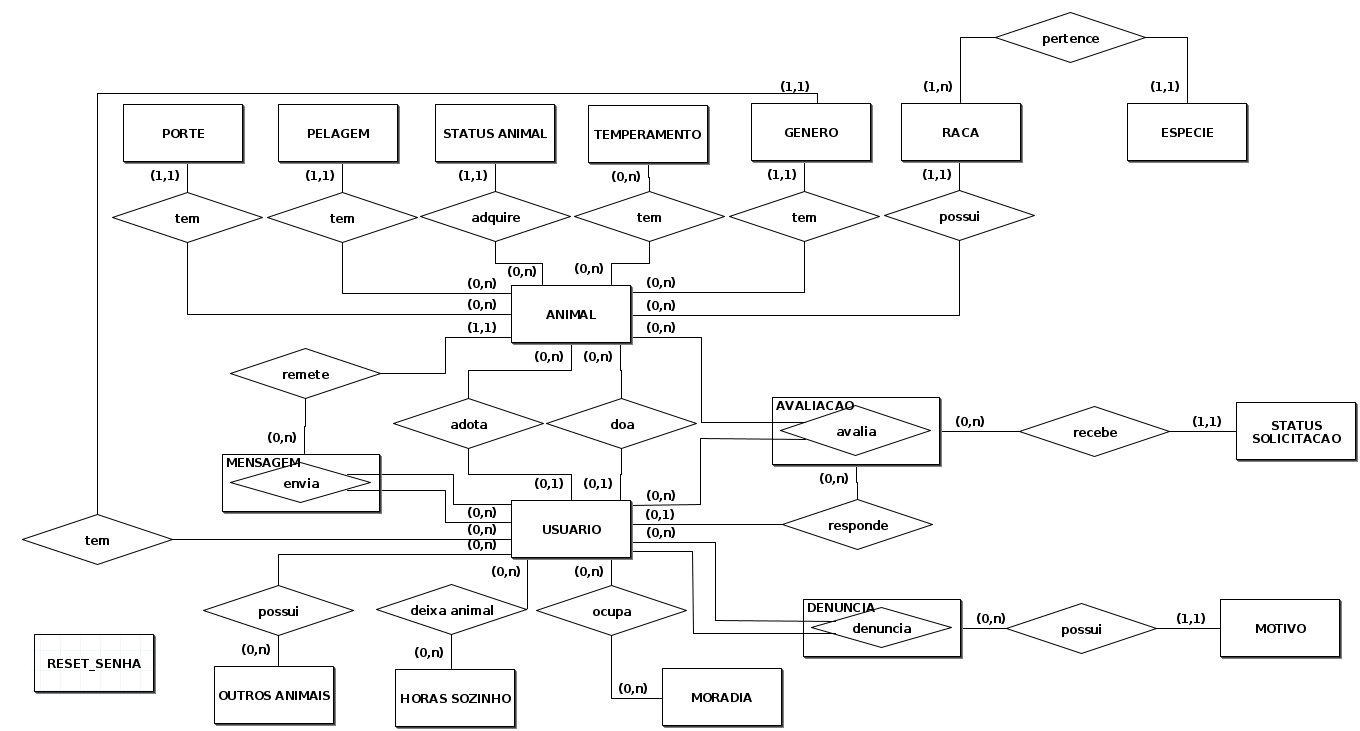
\includegraphics[scale=0.5,angle=90]{imagens/MODELOCONCEITUAL.png}
    \label{mer}
    \fonte{Elaborado pelos autores}
\end{figure}

\begin{figure}
    \centering
    \caption{Modelo Entidade Relacionamento}
    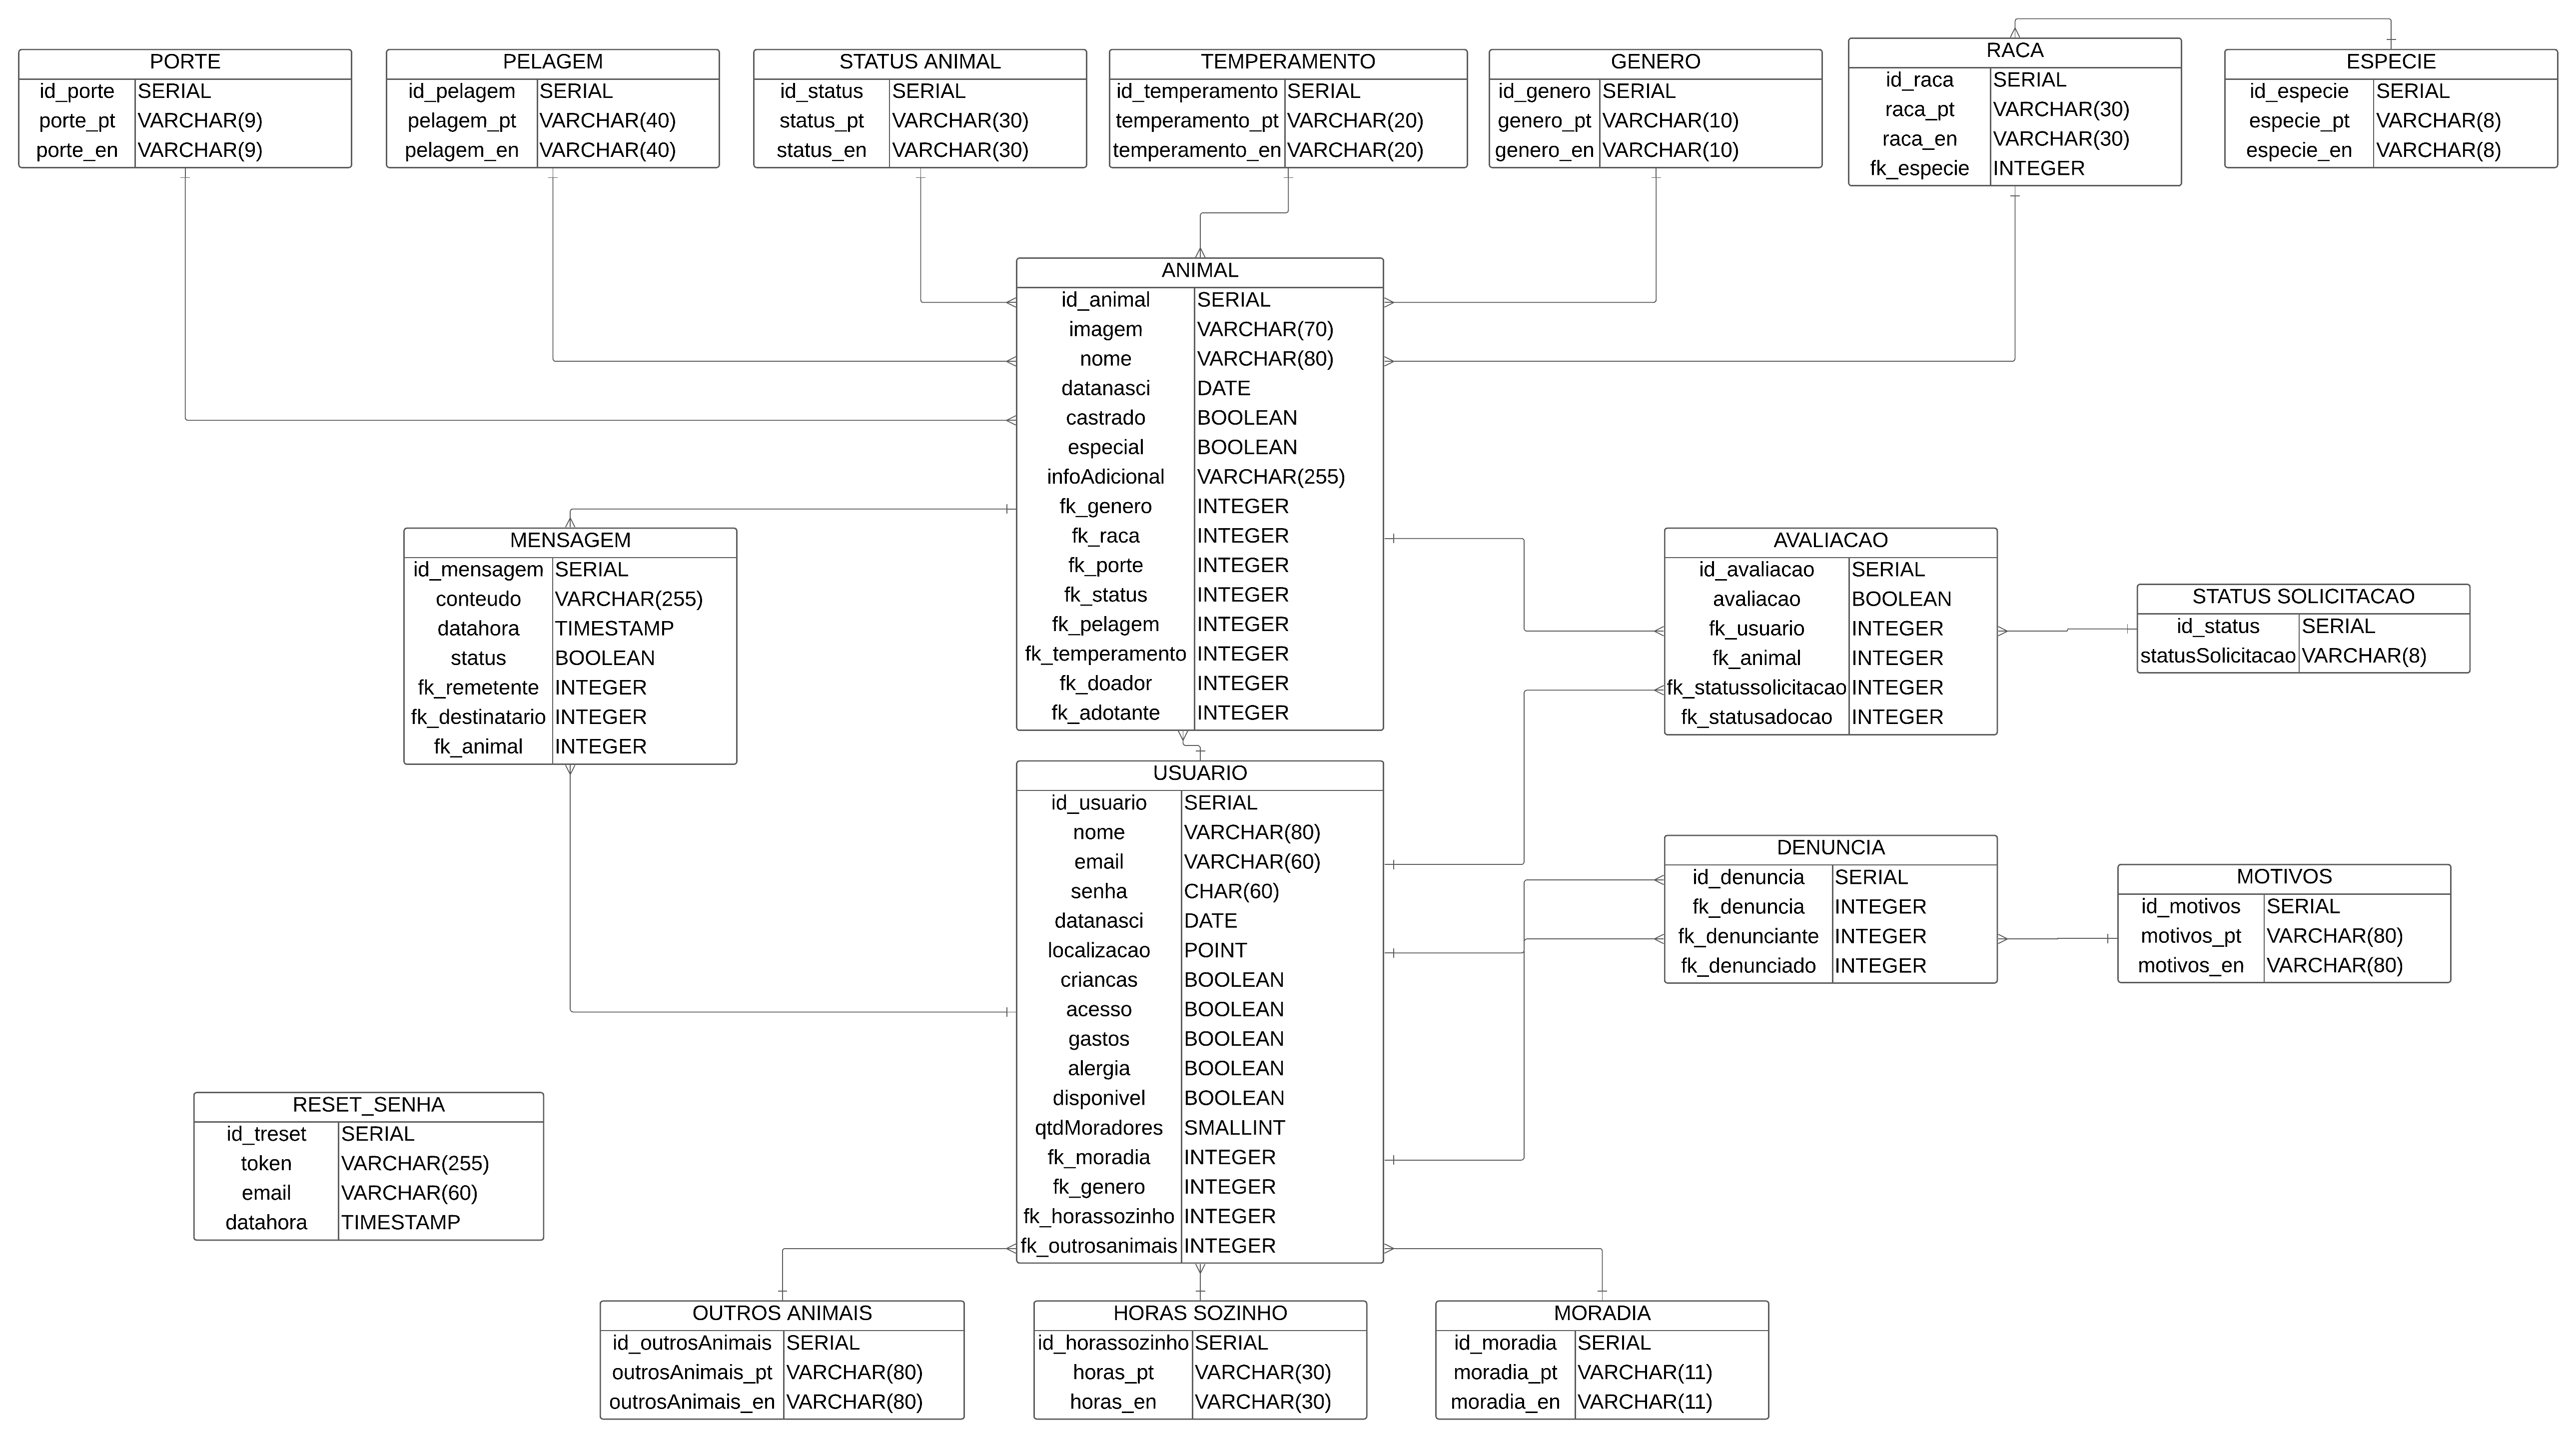
\includegraphics[scale=0.5,angle=90]{imagens/MODELOLOGICO.png}
    \label{der}
    \fonte{Elaborado pelos autores}
\end{figure}

\input{desenvolvimento/texto-desenvolvimento}